\section{Materials and Methods}

\subsection{Workflow and model-development strategy}

\subsubsection{COMSOL source-case pipeline}

The finite element modelling workflow used in this project is a Python-controlled COMSOL Multiphysics pipeline \cite{COMSOLMultiphysicsWebsite}. Model variants and their main parameters are defined in TOML configuration files. These settings are then translated into source-case descriptions, COMSOL Java builders, solver input, post-processing scripts, and compact summary output. The COMSOL implementation was developed as the working continuation of earlier EWS breast-model work, but the model generation used in this report is based on the current COMSOL source-case pipeline.

The public repository is used to store the reproducible parts of the project, such as the code, case definitions, report notes, and compact evaluation output \cite{KuijpersEWSComsolGitHub}. Larger model files generated by COMSOL are kept outside GitHub because they can quickly exceed practical repository storage limits.

\begin{figure}[H]
\centering
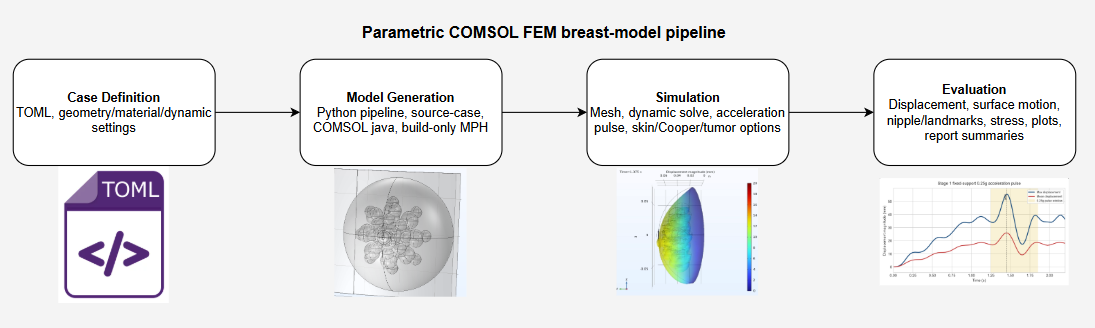
\includegraphics[width=0.95\linewidth]{Figures/model_overviews/model_pipeline_overview.png}
\caption{Overview of the COMSOL EWS FEM pipeline. TOML configuration files define the model variant, after which the Python package generates COMSOL Java builders, build and solve artefacts, post-processing scripts, summary metrics, and report figures.}
\label{fig:mm_pipeline_overview}
\end{figure}

\subsubsection{Thematic development route}

The model was made progressively more complex by adding one modelling component at a time. The development route first established the dynamic excitation, then introduced the posterior support geometry, internal glandular structure, material and skin-layer assumptions, optional support surrogates, and finally tumor/lesion sensitivity. This order keeps the influence of each modelling choice easier to interpret.

The current anatomical reference route combines a volume-preserving xoffset055 chestwall geometry, a realistic glandular lobule distribution, and a matched no-Cooper control. The volumetric skin layer and material-sensitivity cases are treated as active development steps because they strongly affect displacement amplitude. Stage 6 tumor cases are treated as lesion/stiffness sensitivity studies on top of the matched baseline, not as clinical detection validation.

\begin{figure}[H]
\centering
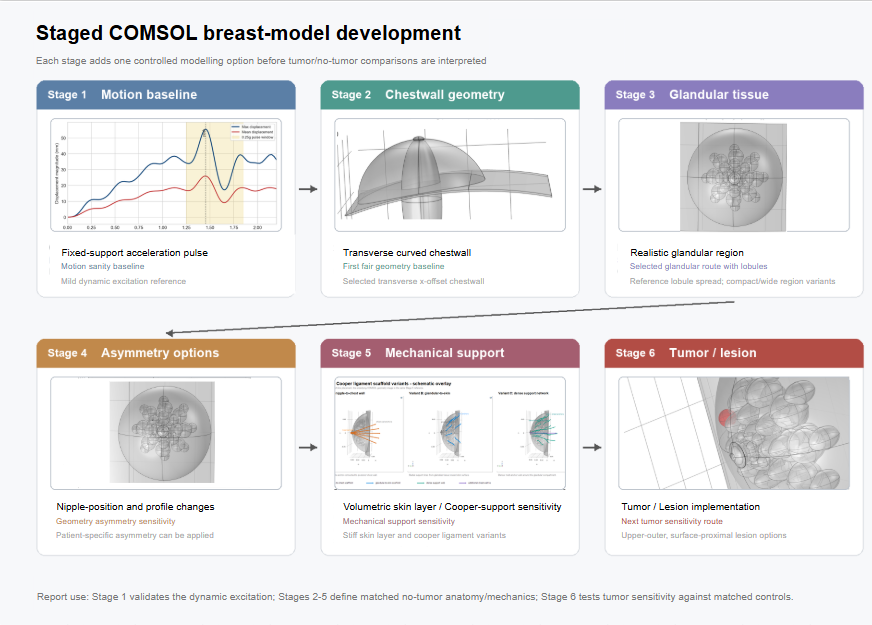
\includegraphics[width=0.95\linewidth]{Figures/model_overviews/Model_stages_overview.png}
\caption{Model-development options used during the COMSOL pipeline development. The model complexity was increased stepwise from motion input and anatomy toward material, support, and tumor sensitivity.}
\label{fig:mm_stage_option_overview}
\end{figure}

\subsubsection{Relation to previous EWS FEM work}

The COMSOL route was developed after earlier EWS FEM work. Ryan Engels' FEBio-based model provided useful context for soft-tissue modelling, dynamic response interpretation, and displacement-based comparison \cite{EngelsEWSReport}. Femke Storm's later Sioux/EWS pipeline provided additional context for skin representation, soft material settings, and a distributed HGO-like adipose reinforcement concept for Cooper-like support \cite{StormEWSReport}. These previous reports are treated as internal project references rather than peer-reviewed validation sources.

The current COMSOL model therefore should not be presented as simply replacing the previous FEBio work. It is a separate implementation route that emphasizes constructive geometry, automated region selections, reproducible case generation, and easier variant management. A short repository and previous-work context is included in \hyperref[sec:appendix_repository_previous_work]{Appendix A}.

\subsection{Anatomical model definition}

\subsubsection{Breast volume and outer geometry}

The breast geometry is parameterized rather than patient-specific. This makes it possible to isolate the effect of controlled model changes, but it should not be presented as a replacement for MRI- or scan-derived patient geometry \cite{Samani2001,Hsu2011,Mazier2024}. The current anatomical route uses a breast volume of approximately 585 mL. This lies in the lower-middle range of the available 100-sample breast-volume dataset and is consistent with using the model as a controlled anatomical baseline rather than as a universal breast shape. The dataset statistics are provided in \hyperref[sec:appendix_volume_summary]{Appendix D}.

\subsubsection{Chestwall geometry and posterior support}

The posterior interface was changed from a simple support surface to a curved chestwall geometry. The selected route uses a transverse xoffset055 chestwall curvature with volume-preserving compensation and automatic alignment of the nipple and glandular structures. Earlier sagittal or combined curvature variants were useful as diagnostic geometry checks, but they were not used as the current report route because they were less stable or less clearly interpretable.

\subsubsection{Glandular tissue distribution}

The reference internal anatomy uses a chestwall-aware realistic glandular lobule distribution. This increased the glandular volume fraction to approximately 24.3\% and is more anatomically informative than the earlier single/simple glandular setup. Compact and wide lobule-spread variants are retained as spatial-distribution sensitivities, while a simplified glandular setup is used only for faster material, skin, and support scouts.

\begin{figure}[H]
\centering
\begin{subfigure}{0.48\linewidth}
\centering
\IfFileExists{Figures/model_pictures/stage3_glandular/stage3_glandular_ref_anterior_offset055.png}{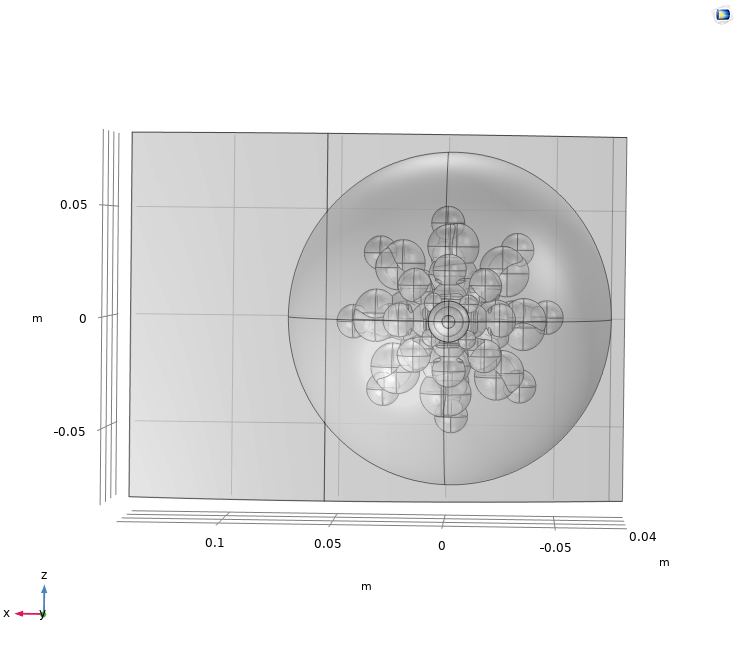
\includegraphics[width=\linewidth]{Figures/model_pictures/stage3_glandular/stage3_glandular_ref_anterior_offset055.png}}{\fbox{\parbox[c][0.24\textheight][c]{0.9\linewidth}{\centering Placeholder: Stage 3 reference anterior view}}}
\caption{Anterior overview}
\end{subfigure}
\hfill
\begin{subfigure}{0.48\linewidth}
\centering
\IfFileExists{Figures/model_pictures/stage3_glandular/stage3_glandular_ref_lateral_slice.png}{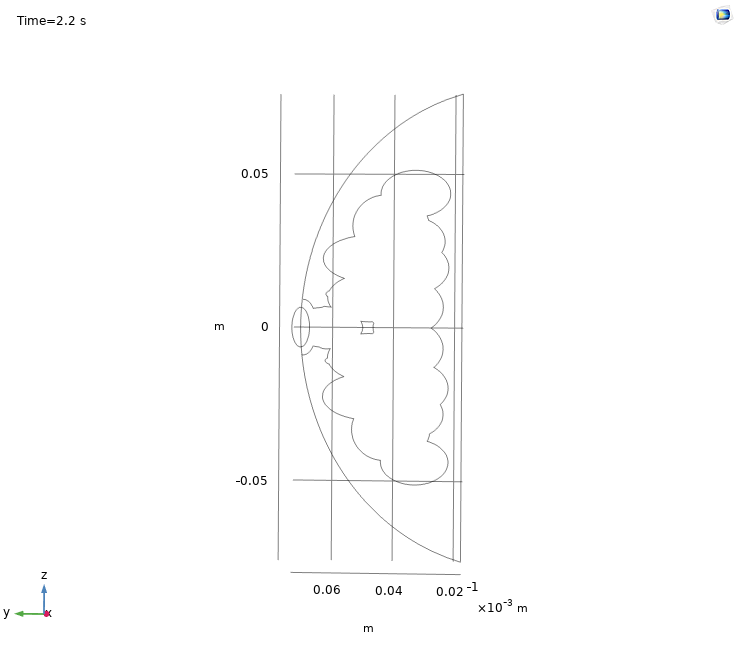
\includegraphics[width=\linewidth]{Figures/model_pictures/stage3_glandular/stage3_glandular_ref_lateral_slice.png}}{\fbox{\parbox[c][0.24\textheight][c]{0.9\linewidth}{\centering Placeholder: Stage 3 reference sagittal slice}}}
\caption{Sagittal slice}
\end{subfigure}
\caption{Current reference geometry used as the anatomical baseline for later sensitivity studies. The figure shows the selected chestwall route combined with the realistic glandular lobule distribution.}
\label{fig:mm_reference_geometry}
\end{figure}

\subsubsection{Asymmetry and nipple-position sensitivity}

Asymmetry and nipple-position changes were implemented as controlled geometry sensitivities. The reference route intentionally keeps these effects disabled, so that profile-asymmetry and nipple-shift variants can later be compared against a clean matched control. These variants are useful for demonstrating parameterization of external anatomy, but they are not yet used as final dynamic evidence.

\subsection{Mechanical model definition}

\subsubsection{Material parameterization}

The source-case material settings contain adipose, glandular, skin, support, and optional tumor/lesion parameters. Literature values for breast soft tissue vary strongly with test protocol, tissue type, loading state, and subject characteristics \cite{Samani2007,Ramiao2016,Teixeira2023,Chen2025}. The material sets are therefore used as controlled sensitivity levels, not as patient-specific calibration.

For interpretability, the Mooney--Rivlin coefficients were converted to an approximate small-strain Young's modulus using \(E \approx 6(C_{10}+C_{01})\). This is only a small-strain comparison metric for a near-incompressible material and does not replace the nonlinear material formulation. The main material sets considered in the Stage 5 development route are summarized in Table~\ref{tab:mm_material_sets}.

\begin{table}[H]
\centering
\caption{Approximate Young's modulus equivalents for the main material sensitivity sets. Values are linearized estimates from the configured Mooney--Rivlin coefficients and are used only to compare stiffness levels.}
\label{tab:mm_material_sets}
\begin{tabular}{p{0.29\linewidth}ccc p{0.27\linewidth}}
\toprule
Material set & Skin \(E\) [kPa] & Adipose \(E\) [kPa] & Glandular \(E\) [kPa] & Use in model \\
\midrule
Current reference & 500 & 3.66 & 10.0 & Stiffer literature-based baseline \\
Volumetric skin & 500 & 3.66 & 10.0 & Same material set with active skin layer \\
Volumetric skin + soft interior & 500 & 1.29 & 2.55 & Internal compliance scout \\
FEBio-like soft set & 14.4 & 1.29 & 2.55 & Historical soft-material comparison \\
Mid-skin sensitivity & 88 & 3.66 or 1.29 & 10.0 or 2.55 & Intermediate skin scout \\
\bottomrule
\end{tabular}
\end{table}

\subsubsection{Volumetric skin layer}

The skin layer was treated as a separate model-development issue. An earlier shell/scaffold representation produced nonphysical surface dimples and bulges during motion and was therefore rejected as a main route. The current route uses a volumetric skin layer around the breast as an active material component. A 1.5 mm layer was selected as the main volumetric-skin test because it is geometrically visible and numerically more robust than an extremely thin volume layer. A 0.1 mm volumetric layer was tested only as a scout because it is not directly equivalent to a 0.1 mm shell and can be more sensitive to mesh quality.

The volumetric skin layer strongly reduces global displacement. Therefore, additional scouts reduced the adipose and glandular stiffness while retaining the skin layer. These soft-interior and FEBio-like material cases were used to test whether displacement amplitude could be increased without removing the anatomically motivated skin representation.

\subsubsection{Cooper/support sensitivity}

Cooper ligament support is currently treated as a support sensitivity rather than an exact anatomical reconstruction. The robust reference case remains the no-Cooper control. The COMSOL Cooper scaffold was implemented as a simplified support surrogate with several direction concepts, including glandular-to-skin, nipple-to-chestwall, and denser support variants. In the simple-gland scout route, these variants produced only small global displacement changes and are therefore not treated as a validated Cooper model.

Femke's previous FEBio/Sioux workflow used an HGO-style anisotropic adipose reinforcement as a more distributed Cooper-like concept \cite{StormEWSReport}. A COMSOL build-only probe for a similar HGO-like adipose feature did not create a usable HGO material feature in the generated model. This route was therefore left as future work. The report should describe the current Cooper implementation as diagnostic/support sensitivity only.

\subsubsection{Tumor/lesion material overlay}

The current Stage 6 tumor route uses an analytic spherical material overlay rather than a separate segmented tumor domain. A \texttt{tumor\_mask} is defined from radius and position parameters. Inside that mask, density and stiffness-related material expressions are modified locally. This approach avoids fragile Boolean geometry operations while allowing controlled tumor size, stiffness, and location studies. It does not create a separate \texttt{mat\_tumor} material or separate tumor domain.

The initial lesion sizes are 6 mm, 12 mm, and 20 mm diameter. These span small early lesions, a mid-range screening-style lesion, and an upper T1-size diagnostic sensitivity; they also align with earlier DIET phantom work that tested 5, 10, and 20 mm stiff inclusions \cite{NCI_TNM,Kashif2013}. The first location set includes central, subareolar, posterior/chestwall-proximal, and upper-outer candidates. The upper-outer candidate is emphasized because breast-cancer quadrant studies report this as the most frequent tumor site \cite{Rummel2015,Yu2017}. Additional surface-proximal candidates were added because tumor-to-skin or tumor-to-dermis distance is clinically evaluated in superficial breast tumors \cite{Brandao2023,Yur2023}.

Tumor shape is kept spherical in the current implementation. Imaging descriptors such as round, oval, irregular, and spiculated masses are clinically relevant in BI-RADS terminology \cite{ACRBIRADS,UCLABIRADS}, but ellipsoidal or irregular lesion shapes would require extending the analytic mask or adding separate visual geometry. Those shapes are therefore treated as future Stage 6B sensitivity cases rather than current results.

\begin{figure}[H]
\centering
\begin{subfigure}{0.48\linewidth}
\centering
\IfFileExists{Figures/model_pictures/stage6_tumor/stage6_tumor_small_upper_outer_leftlateral.png}{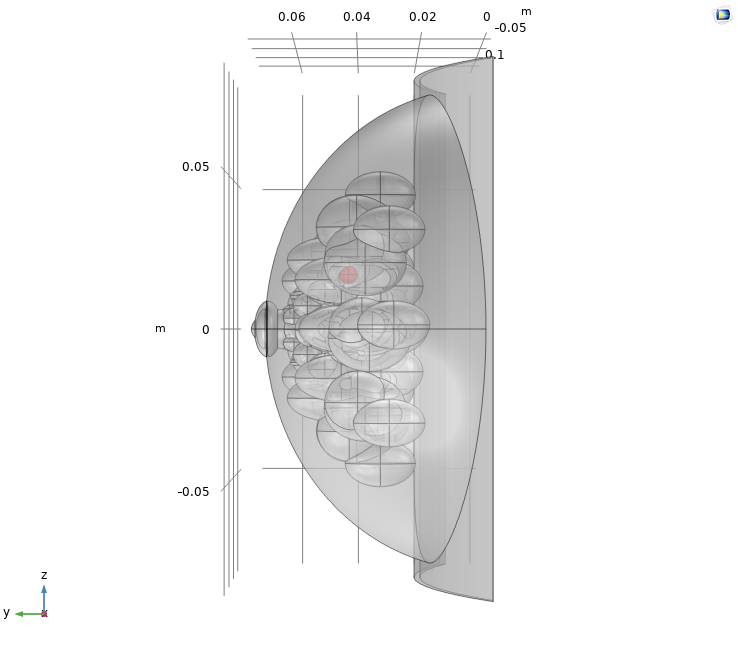
\includegraphics[width=\linewidth]{Figures/model_pictures/stage6_tumor/stage6_tumor_small_upper_outer_leftlateral.png}}{\fbox{\parbox[c][0.24\textheight][c]{0.9\linewidth}{\centering Placeholder: small upper-outer tumor view}}}
\caption{Small upper-outer candidate}
\end{subfigure}
\hfill
\begin{subfigure}{0.48\linewidth}
\centering
\IfFileExists{Figures/model_pictures/stage6_tumor/stage6_tumor_large_central_sideview.png}{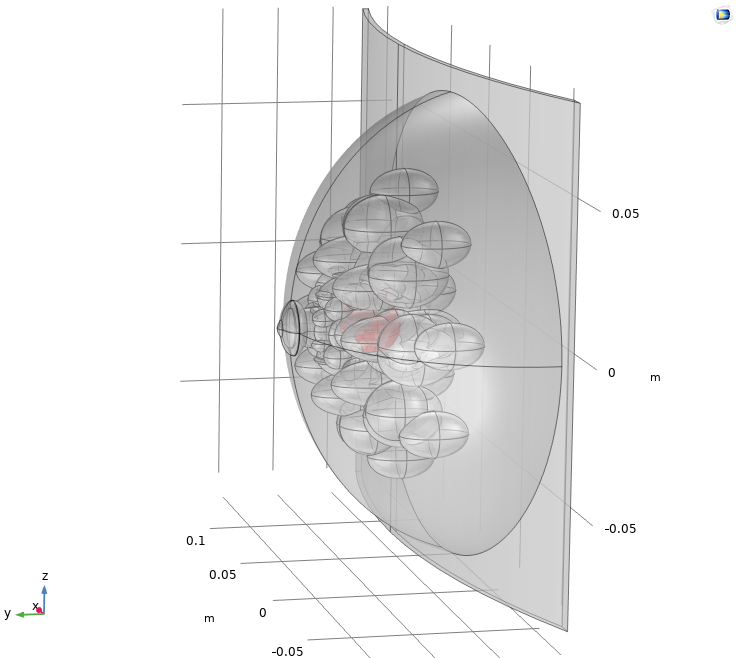
\includegraphics[width=\linewidth]{Figures/model_pictures/stage6_tumor/stage6_tumor_large_central_sideview.png}}{\fbox{\parbox[c][0.24\textheight][c]{0.9\linewidth}{\centering Placeholder: large central tumor view}}}
\caption{Large central candidate}
\end{subfigure}
\caption{Visual examples of the Stage 6 spherical tumor-mask screening route. These images document placement and scale; quantitative interpretation depends on completed tumor-mask and surface-response metrics.}
\label{fig:mm_stage6_tumor_visual}
\end{figure}

\subsection{Dynamic excitation}

\subsubsection{Fixed-support acceleration pulse}

The original standard transient input was a fixed-support acceleration pulse with amplitude 0.25g, duration 0.60 s, and mass damping alpha = 60 s$^{-1}$. This input is intended as a mild platform- or torso-like acceleration for controlled model comparison. It should not be described as a direct physical reproduction of a jump or as an exact Early Warning Scan protocol. Higher-amplitude cases, including 1.00g and 1.25g, were used as diagnostic excitations to increase observable motion and to study material sensitivity.

\subsubsection{Prescribed support-displacement scout}

Because the fixed-support acceleration pulse did not always produce intuitive external motion, an additional Stage 5.1 motion scout was introduced. In this route, gravity first brings the breast to a hanging position while the chestwall/support is held fixed. After this preload phase, a smooth prescribed support displacement moves the support upward and back down. This scout is closer to a controlled platform-displacement interpretation than the acceleration-pulse route, but it is still a diagnostic model input rather than a validated human jump protocol.

Several support-displacement amplitudes and durations were explored. The purpose was not to replace the baseline immediately, but to determine whether a support-displacement input can produce smoother and more interpretable surface motion. These runs should be reported as motion-input scouts until a final amplitude, duration, damping setting, and post-processing route are selected.

\subsection{Mesh, build, and solver checks}

The pipeline supports generate-only, build-only, full run, and postprocess-only workflows. For new geometry or lesion cases, build-only is used first to verify geometry construction, selections, source-case expansion, and generated Java output without starting a heavy solve. This is especially important for Stage 6, where tumor location must be checked visually and numerically before interpreting displacement or stress results.

The current report-oriented COMSOL cases use a free tetrahedral mesh with a source-case characteristic length setting of \texttt{ls = 0.005} m, corresponding to approximately 5 mm. The mesh density hint is set to 125 and the active dynamic cases use second-order elements. These settings are a practical compromise between resolving the breast surface, nipple region, glandular lobules, and volumetric skin layer while keeping overnight dynamic solves feasible on the available laptop/workstation. A full mesh-convergence study was not completed, so the current mesh should be interpreted as a verified working mesh for model-development comparisons rather than as a final discretization-independent solution.

\begin{figure}[H]
\centering
\begin{subfigure}{0.48\linewidth}
\centering
\IfFileExists{Figures/model_pictures/mesh/mesh_overview.png}{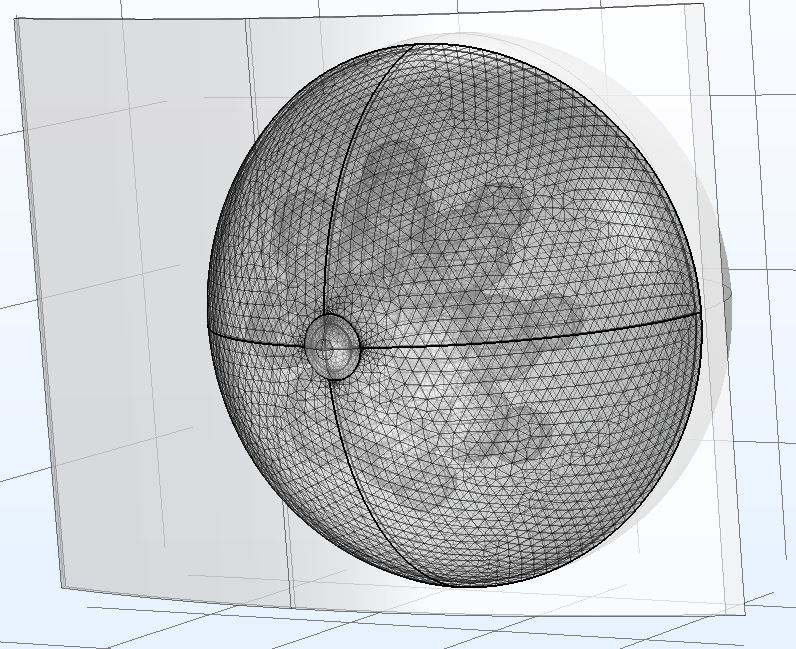
\includegraphics[width=\linewidth]{Figures/model_pictures/mesh/mesh_overview.png}}{\fbox{\parbox[c][0.24\textheight][c]{0.9\linewidth}{\centering Placeholder: mesh overview}}}
\caption{Global mesh overview}
\end{subfigure}
\hfill
\begin{subfigure}{0.48\linewidth}
\centering
\IfFileExists{Figures/model_pictures/mesh/mesh_zoomed_nipple_view.png}{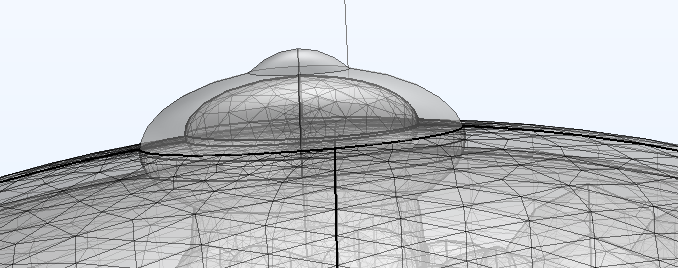
\includegraphics[width=\linewidth]{Figures/model_pictures/mesh/mesh_zoomed_nipple_view.png}}{\fbox{\parbox[c][0.24\textheight][c]{0.9\linewidth}{\centering Placeholder: local nipple mesh}}}
\caption{Nipple-region refinement}
\end{subfigure}
\caption{Representative free tetrahedral mesh used for the current COMSOL model-development route. The images document the working discretization and local surface resolution used in build and solve checks.}
\label{fig:mm_mesh_overview}
\end{figure}

\subsection{Post-processing and evaluation metrics}

The post-processing route exports breast, glandular, adipose, and tumor-mask metrics when available. The main quantities are total breast volume, glandular volume fraction, average and maximum displacement, signed surface displacement, nipple/landmark displacement, average and maximum von Mises stress, tissue stress, and time-series evolution. For tumor cases, additional mask-based metrics include tumor volume, tumor-region displacement, and tumor-region stress.

For selected solve-only scout cases, the COMSOL GUI was also used as a manual fallback post-processing route. Derived Values were evaluated on the breast-union domain using the same dataset and stored solution times for each model. The exported quantities were volume averages and maxima of \texttt{solid.disp} and \texttt{solid.mises}. For EWS-oriented scout comparisons, additional surface exports were made on the free outer breast surface, including \texttt{solid.disp}, displacement components \texttt{u}, \texttt{v}, and \texttt{w}, and \texttt{solid.mises}. These manual CSV exports were used only when the automated post-processing batch route was unreliable; they do not replace the full automated surface, landmark, or tumor-mask exports for final case sets.

For the EWS application, global displacement is only a context metric. The most relevant quantities are surface displacement and local surface-response differences between matched no-tumor and tumor cases. Therefore, later tumor interpretation should focus on outer-surface maps, signed vertical displacement, local tumor-region surface response, and matched difference maps rather than only on global maximum displacement.

\subsection{Reproducibility and data management}

The repository is intended to preserve the reproducible parts of the project: source code, active TOML files, report notes, compact CSV summaries, plotting scripts, figures, and documentation. Large generated MPH files, COMSOL recovery files, build folders, solve folders, and raw surface exports are not suitable for GitHub and are kept as local or removable artefacts. This separation is important because the full COMSOL outputs can become several gigabytes per case, while the report conclusions only require the TOML provenance, compact post-processing tables, plots, and selected screenshots.

The final report therefore distinguishes between report-ready evidence, diagnostic/scout results, and local generated artefacts. TOML files define the model cases, compact post-processing outputs support quantitative comparisons, and screenshots document geometry and visual checks. Heavy solve artefacts are only retained while they are still needed for inspection or additional post-processing.
